% generated by scripts/pkl_to_latex.py
% source PKL : tscan_v1_L8_Ne8_U10_mode-uniform_nmin2_solver-gcg_sz0_restarts2_iter200_kmax4_tol1em09_t0.05to2_N20-d03538a42051.pkl
% scan type  : tscan
% state      : gs
% requires   : \usepackage{pgfplots} \pgfplotsset{compat=1.18}
% colours match the matplotlib PDF (tab10 cycle)
\definecolor{gmeC0}{HTML}{1F77B4}
\definecolor{gmeC1}{HTML}{FF7F0E}
\definecolor{gmeC2}{HTML}{2CA02C}
\definecolor{gmeC3}{HTML}{D62728}
\definecolor{gmeC4}{HTML}{9467BD}
\definecolor{gmeC5}{HTML}{8C564B}
\definecolor{gmeC6}{HTML}{E377C2}
\definecolor{gmeC7}{HTML}{17BECF}

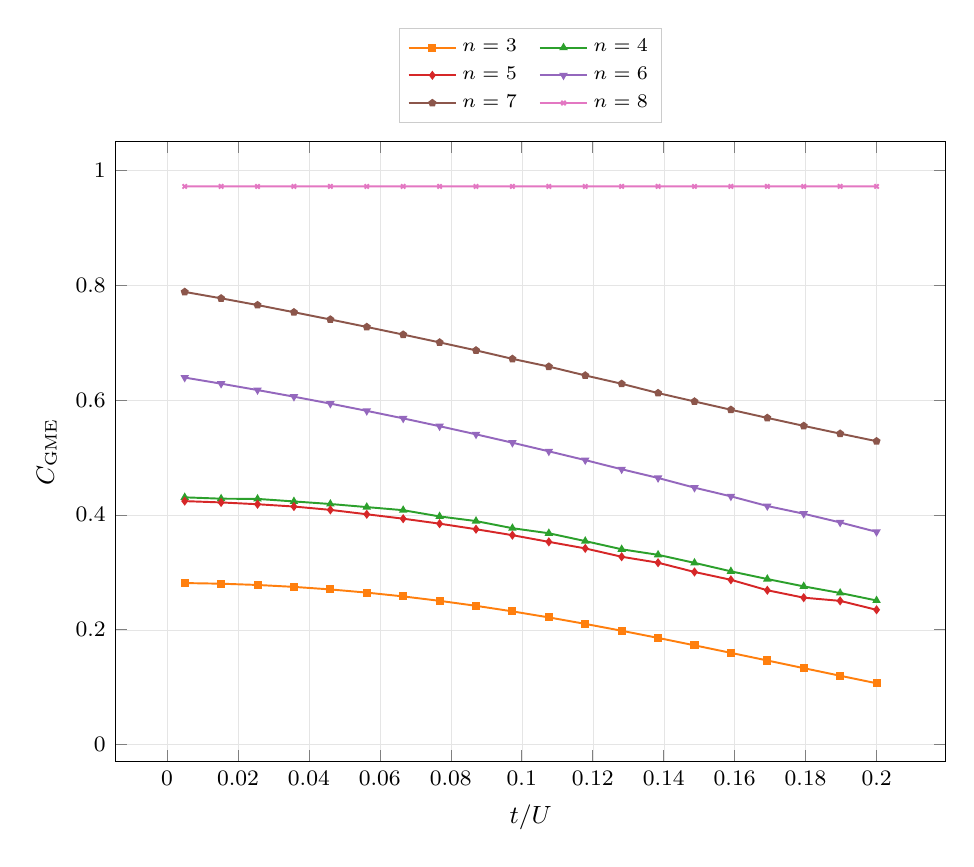
\begin{tikzpicture}
  \begin{axis}[
    width=\columnwidth,
    height=0.78\columnwidth,
    xlabel={$t/U$},
    ylabel={$C_{\mathrm{GME}}$},
    grid=both,
    grid style={line width=.1pt, draw=gray!20},
    tick label style={font=\footnotesize\rmfamily, /pgf/number format/fixed},
    label style={font=\small\rmfamily},
    scaled ticks=false,
    legend style={font=\scriptsize\rmfamily, draw=gray!40, at={(0.5,1.03)}, anchor=south, /tikz/every even column/.append style={column sep=6pt}},
    legend cell align={left},
    legend columns=2,
    ymin=-0.03,
    ymax=1.05,
  ]
    \addplot[color=gmeC1, mark=square*, mark size=1.1pt, line width=0.7pt] coordinates {
        (0.005,0.281155) (0.015263,0.280054) (0.025526,0.277837) (0.035789,0.274506)
        (0.046053,0.270067) (0.056316,0.264526) (0.066579,0.2579) (0.076842,0.250218)
        (0.087105,0.241521) (0.097368,0.231872) (0.107632,0.22135) (0.117895,0.210057)
        (0.128158,0.198107) (0.138421,0.185627) (0.148684,0.17275) (0.158947,0.159605)
        (0.169211,0.146318) (0.179474,0.133001) (0.189737,0.119754) (0.2,0.106664)
    };
    \addlegendentry{$n=3$}
    \addplot[color=gmeC2, mark=triangle*, mark size=1.1pt, line width=0.7pt] coordinates {
        (0.005,0.430453) (0.015263,0.428094) (0.025526,0.427701) (0.035789,0.423302)
        (0.046053,0.418836) (0.056316,0.413455) (0.066579,0.408049) (0.076842,0.397179)
        (0.087105,0.389122) (0.097368,0.376698) (0.107632,0.367884) (0.117895,0.354248)
        (0.128158,0.339978) (0.138421,0.33033) (0.148684,0.316331) (0.158947,0.301589)
        (0.169211,0.288156) (0.179474,0.275384) (0.189737,0.263864) (0.2,0.250805)
    };
    \addlegendentry{$n=4$}
    \addplot[color=gmeC3, mark=diamond*, mark size=1.1pt, line width=0.7pt] coordinates {
        (0.005,0.423856) (0.015263,0.421577) (0.025526,0.418428) (0.035789,0.414421)
        (0.046053,0.408606) (0.056316,0.400941) (0.066579,0.393282) (0.076842,0.384602)
        (0.087105,0.374923) (0.097368,0.364554) (0.107632,0.352913) (0.117895,0.341503)
        (0.128158,0.326948) (0.138421,0.316601) (0.148684,0.300465) (0.158947,0.286837)
        (0.169211,0.268631) (0.179474,0.2557) (0.189737,0.250143) (0.2,0.234574)
    };
    \addlegendentry{$n=5$}
    \addplot[color=gmeC4, mark=triangle*, mark size=1.1pt, mark options={rotate=180}, line width=0.7pt] coordinates {
        (0.005,0.639038) (0.015263,0.628377) (0.025526,0.617281) (0.035789,0.605726)
        (0.046053,0.593659) (0.056316,0.581059) (0.066579,0.567946) (0.076842,0.554316)
        (0.087105,0.54018) (0.097368,0.52557) (0.107632,0.510568) (0.117895,0.495257)
        (0.128158,0.479362) (0.138421,0.464171) (0.148684,0.447298) (0.158947,0.432193)
        (0.169211,0.415333) (0.179474,0.401889) (0.189737,0.386733) (0.2,0.370347)
    };
    \addlegendentry{$n=6$}
    \addplot[color=gmeC5, mark=pentagon*, mark size=1.1pt, line width=0.7pt] coordinates {
        (0.005,0.788202) (0.015263,0.777014) (0.025526,0.765277) (0.035789,0.752791)
        (0.046053,0.740171) (0.056316,0.727185) (0.066579,0.713865) (0.076842,0.70025)
        (0.087105,0.686387) (0.097368,0.671598) (0.107632,0.658144) (0.117895,0.642725)
        (0.128158,0.628221) (0.138421,0.612032) (0.148684,0.597406) (0.158947,0.582973)
        (0.169211,0.568783) (0.179474,0.554913) (0.189737,0.5414) (0.2,0.52819)
    };
    \addlegendentry{$n=7$}
    \addplot[color=gmeC6, mark=x, mark size=1.1pt, line width=0.7pt] coordinates {
        (0.005,0.971886) (0.015263,0.971886) (0.025526,0.971886) (0.035789,0.971886)
        (0.046053,0.971887) (0.056316,0.971887) (0.066579,0.971887) (0.076842,0.971888)
        (0.087105,0.971888) (0.097368,0.97189) (0.107632,0.971891) (0.117895,0.971892)
        (0.128158,0.971894) (0.138421,0.971897) (0.148684,0.9719) (0.158947,0.971903)
        (0.169211,0.971906) (0.179474,0.97191) (0.189737,0.971914) (0.2,0.971918)
    };
    \addlegendentry{$n=8$}
  \end{axis}
\end{tikzpicture}
